\documentclass[12pt]{beamer}
\usepackage[utf8]{vietnam}
\usepackage{lmodern}
\usepackage{animate}
\usepackage{wrapfig}
\usetheme{metropolis}

\begin{document}
	\author{Đặng Quang Anh - Cao Việt Tùng}
	\title{TABU SEARCH}
	\date{Tháng 6 2021}
	%\subtitle{}
	%\logo{}
	%\institute{}
	%\date{}
	%\subject{}
	%\setbeamercovered{transparent}
	%\setbeamertemplate{navigation symbols}{}
	\maketitle
	
	\frame<beamer>{
		\frametitle{Outline}
		\tableofcontents
	}

	\section{Search Space and Neighbor Structure}
	\begin{frame}
		\frametitle{Search Space and Neighbor Structure}
		\begin{itemize}
			\item Search Space - Không gian tìm kiếm: Là khoảng không gian của tất cả các giải pháp có thể xem xét (ghé thăm) trong quá trình tìm kiếm.
			\item Neighbor Structure - Cấu trúc vùng lân cận: Là một tập con của Search Space định nghĩa bởi\\
					$N(S) = \{ $giải pháp thu được bằng cách áp dụng một biến đổi cục bộ duy nhất cho S$ \}$
		\end{itemize}
	\end{frame}

	\begin{frame}
		\frametitle{Search Space and Neighbor Structure}
		Ví Dụ:\\
		Với bài toán TSP:\\
		\begin{itemize}
			\item Search Space là tập hợp tất cả cách cách đi khả thi của người bán hàng
			\item Với một cách đi S của người bán hàng (giả sử là 1-2-3-4-5) thì bằng cách đổi chỗ 2 thành phố bất kì trong cách đi trên ta thu được một tập hợp các nước đi và đó là Neighbor Structure của S.
		\end{itemize}
	\end{frame}
	
	\section{Tabus}
	\begin{frame}
		\frametitle{Tabus}
		Giải thuật leo đồi(Hill Climbing): Ở mỗi lần lặp, tìm giải pháp tốt hơn giải pháp tốt hơn giải pháp hiện tại trong vùng lân cận (Neighbor Structure), nếu không có thì thuật toán dừng lại.Điều đó dẫn đến thuật toán có thể bị kẹt lại tối ưu cục bộ.\\
		Ví dụ:\\
		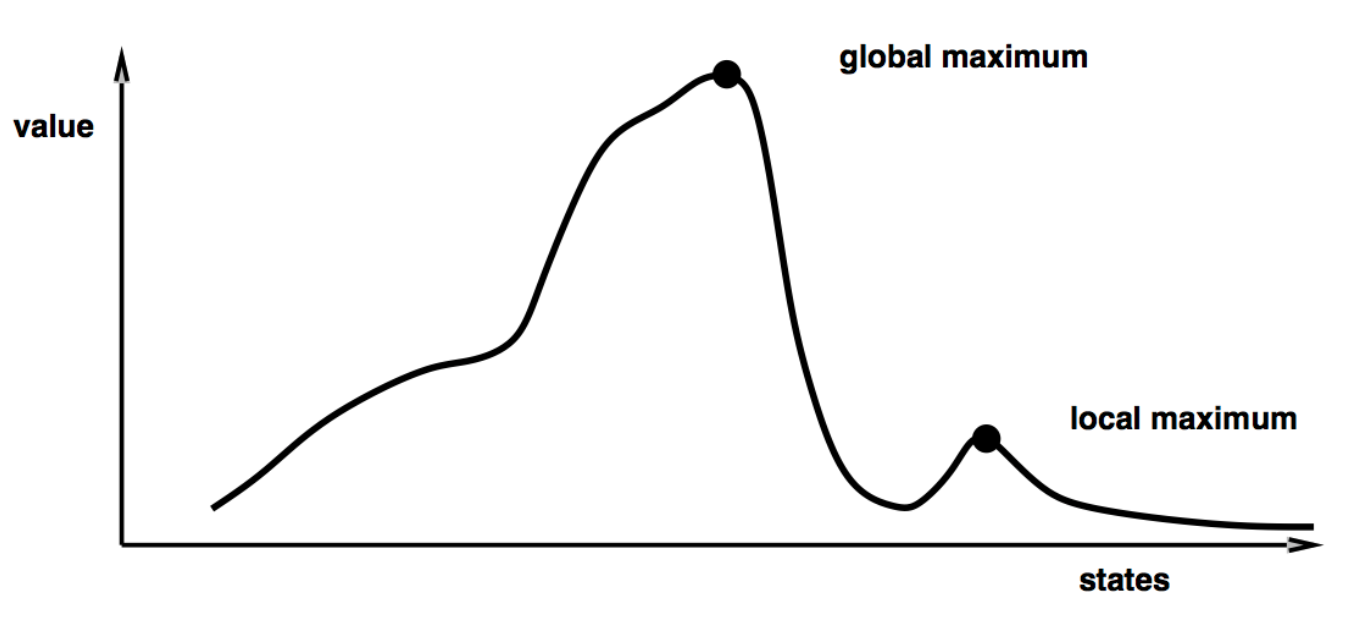
\includegraphics[scale=0.4]{HillClimbing.png}\\
	\end{frame}

	\begin{frame}
		\frametitle{Tabus}
		Tabu Search cho phép di chuyển khỏi tối ưu cục bộ bằng các bước đi không cải thiện.\\
		Khi việc đó xảy ra, cần phải làm gì đó để ngăn việc tìm kiếm lần theo các bước của chính nó về điểm xuất phát.\\
		Điều này có thể có nghĩa là không cho phép việc tìm kiếm quay trở lại điểm đã ghé thăm gần đây trong không gian tìm kiếm hoặc không cho phép các bước di chuyển gần bị đảo ngược.\\
		Ta thực hiện việc này bằng cách sử dụng Tabus.
	\end{frame}

	\begin{frame}
		\frametitle{Tabus}
		Một bước đi được gọi là Tabu nếu nó đã được đi trong vòng một số lần tìm kiếm trước đó.\\
		Tabus được lưu trữ trong bộ nhớ ngắn hạn của cuộc tìm kiếm (tabu list)\\
		Ví Dụ:\\
		Trong bài toán job shop scheduling, ta có thể định nghĩa tabus theo nhiều cách.Nếu một công việc $j$ vừa được chuyển từ vị trí $p_1$ sang vị trí $p_2$, ta có thể khai báo tabu moves đặc biệt $j$ về vị trí $p_1$ từ vị trí $p_2$ và ghi lại điều này trong bộ nhớ ngắn hạn dưới dạng bộ ba $(j, p_2, p_1)$.Một tabu mạnh hơn sẽ liên quan tới việc cấm di chuyển $j$ trở lại $p_1$ (không tính đến vị trí hiện tại của nó) và được ghi lại là $(j, p_1)$. Một tabu mạnh hơn nữa sẽ không cho phép di chuyển $j$, và sẽ đơn giản được ghi chú là $(j)$.
	\end{frame}
	
	\section{Aspiration Criterion}
	\begin{frame}
		\frametitle{Aspiration Criterion}
		Như đã nói ở trên, Tabu Search cho phép các bước di chuyển mà không cải thiện để có thể ra khỏi tối ưu cục bộ.\\
		Đó là khi Aspiration Criterion(Tiêu chí khát vọng) được sử dụng.\\
		Ví dụ:\\
		Ta đang ở trạng thái $x$, trong khi đó $x^*$ là giải pháp tốt nhất cho đến hiện tại.\\
		Bước đi $x'$ là bước đi không cải thiện nếu $P(x') \le P(x^*)$ và bước đi này vẫn được chấp thuận nếu $P(x') \ge P(x)$
	\end{frame}

	\section{Tabu Search trong bài toán TSP}
	\begin{frame}
		\frametitle{Tabu Search trong bài toán TSP}
			\begin{wrapfigure}{l}{5cm}
				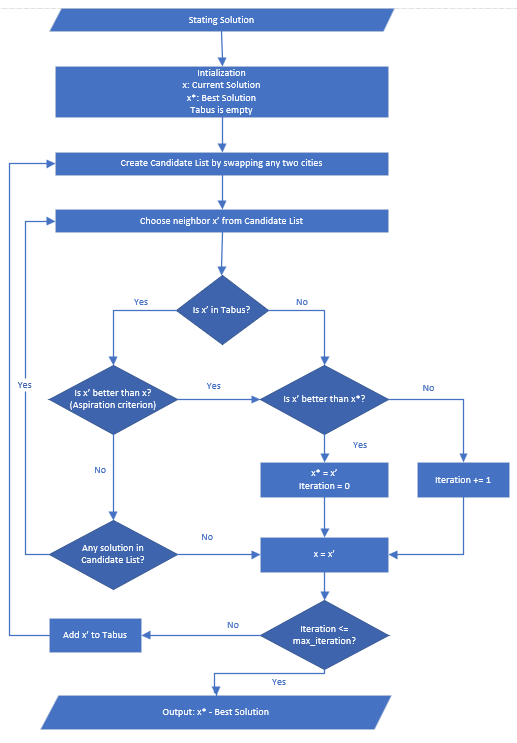
\includegraphics[width=5cm]{Tabu.png}
			\end{wrapfigure}
		Áp dụng Tabu Search vào bài toán TSP\\
		a\\
		a\\
		a\\
		a\\
		a\\
		a\\
		a\\
		a\\
		a\\
		a\\
	\end{frame}
\end{document}